\documentclass[]{beamer}
\usepackage{xmpmulti}
\usepackage{psfrag}
\usepackage{xcolor}


\mode<presentation>
{\usetheme{Boadilla}  % very plain
}

\usepackage{xcolor}

\usepackage{amssymb,amsmath,amsthm}
\usepackage{boxedminipage}

\setbeamercolor{uppercol}{fg=teal,bg=lightgray}%
\setbeamercolor{lowercol}{fg=olive,bg=lightgray!50}%

\newcommand{\curr}{\mathtt{current}}
\newcommand{\mos}{\mathtt{m}}
\newcommand{\move}{\mathtt{lmove}}
\newcommand{\nmove}{\mathtt{nmove}}

\title[]{Asymmetric Crypto with OpenSSL}

\author{Giuseppe Persiano}

\institute[UNISA]{%
Universit\`a di Salerno\\ \qquad \\
}

\date[November 2020]{November, 2020}

\begin{document}

{
\begin{frame}
  \titlepage
\end{frame}
\begin{frame}
\frametitle{RSA with OpenSSL}
\begin{block}{Key Generation}
\begin{itemize}
\item {\tt openssl genpkey}: generate private key
\item {\tt -aes256}: encryption algorithm used to armor the private key
\item {\tt -algorithm RSA}: public-key encryption scheme
\item {\tt -pkeyopt rsa\_keygen\_bits:2048} specify option for the key.

In this case the number of bits

\item {\tt -out: } file that will store the key
\end{itemize}
\end{block}

\vskip 1cm

The key is stored in the {\tt PKCS\#8} format

Encrypted using {\tt PBKDF2} with {\tt hmacWithSHA256} as a PRF
\vskip .3cm
Public exponent: {\tt 65537 (0x10001)}

{\tt -pkeyopt rsa\_keygen\_pubexp:} to modify 
\end{frame}

\begin{center}
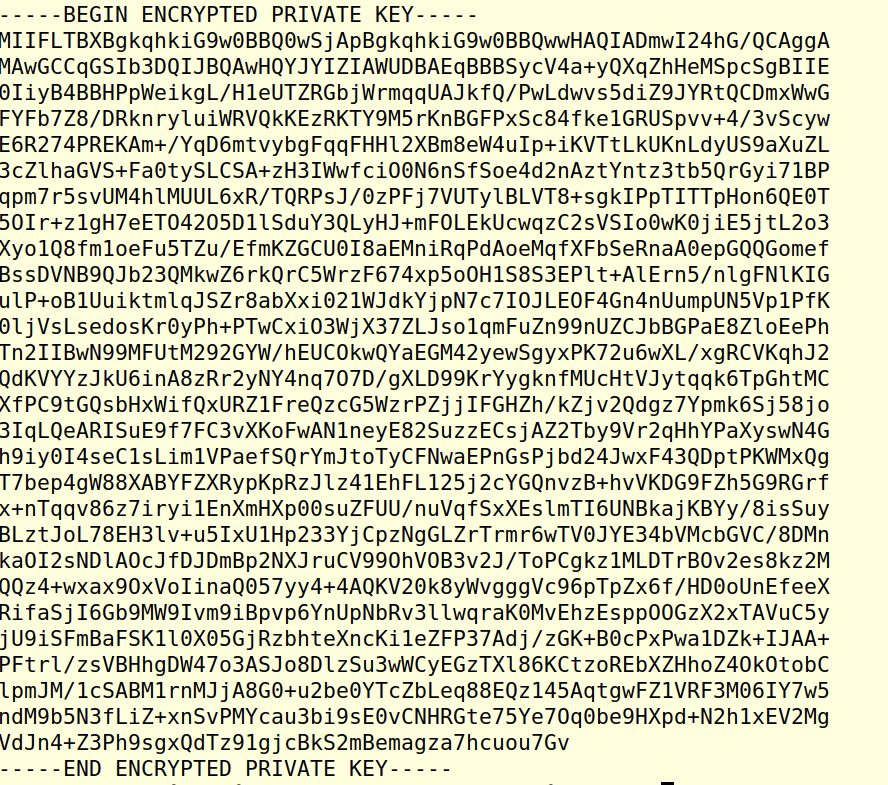
\includegraphics[width=3.5in]{imgs/rsaPrivate8.png}
\end{center}


\vfill

Not very informative

\begin{frame}
\begin{block}{Key Generation: Obsolete}

\begin{itemize}
\item {\tt openssl genrsa}
\item {\tt -aes128}: encryption algorithm used to armor the private key
\item {\tt -out } file that will store the key
\item {\tt len} in bits of the key
\end{itemize}
\centerline{\color{blue} \tt openssl genrsa -aes128 -out giuperPrivateRSA.pem 2048}

\end{block}
\vskip .5cm
\vskip .5cm
The key is stored in the {\tt PKCS\#1} format

\vskip .3cm
Public exponent: {\tt 65537 (0x10001)}

\end{frame}

\begin{center}
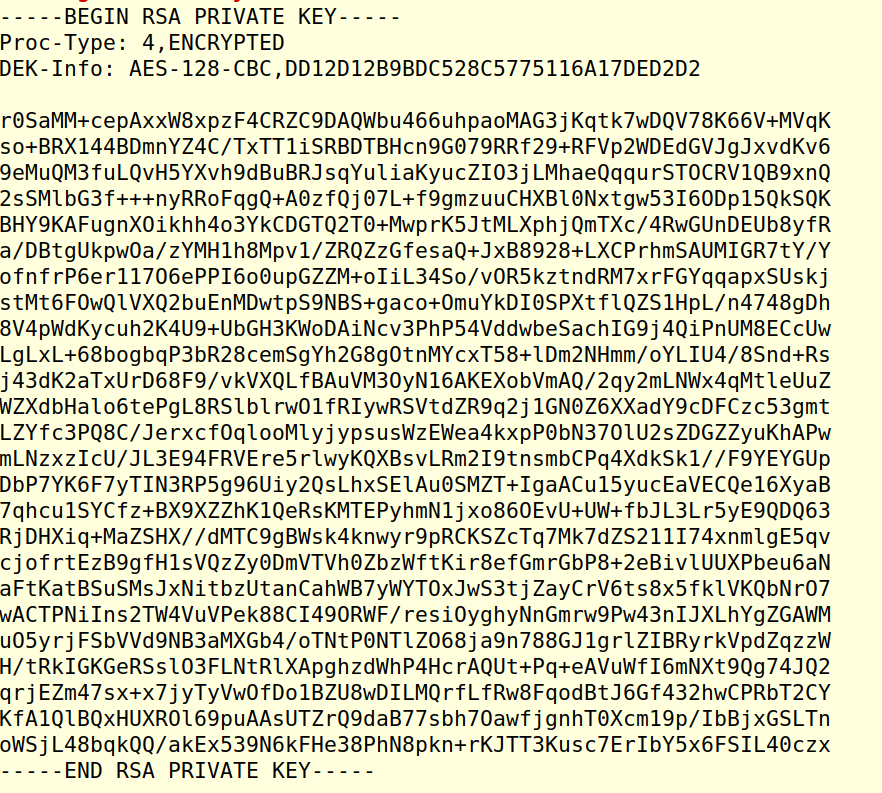
\includegraphics[width=3.5in]{imgs/rsaPrivate1.png}
\end{center}


\vfill

Not very informative

\begin{frame}
\frametitle{What is in a key}

\centerline{\color{blue} \tt openssl rsa -text -in giuperPrivateRSA.pem -noout}

\begin{center}
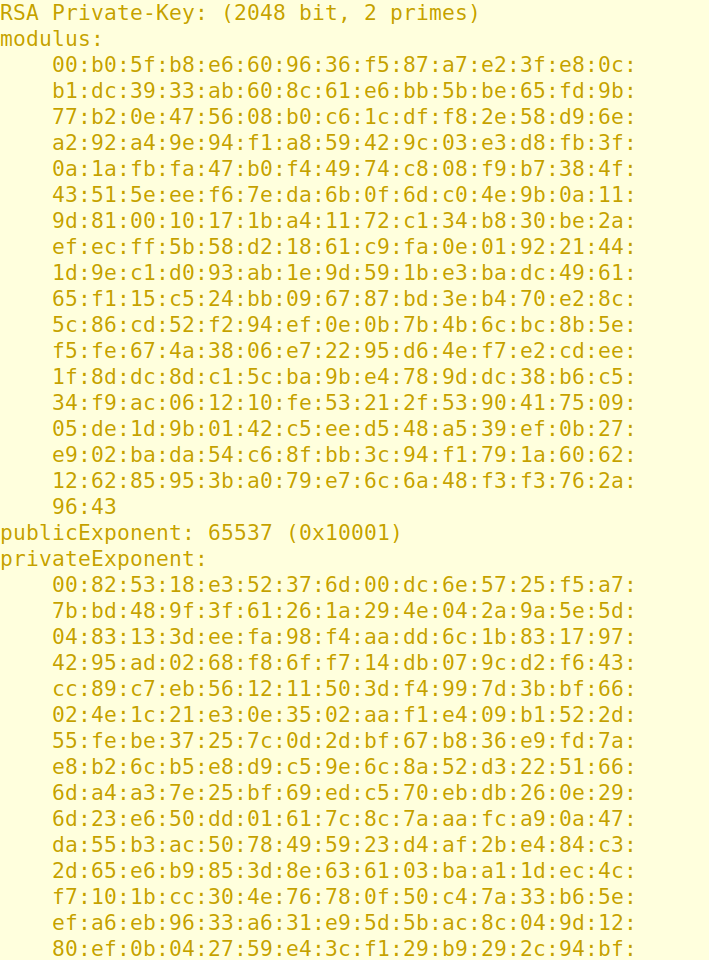
\includegraphics[width=3in]{imgs/rsaPrivateInform.png}
\end{center}
\end{frame}

\begin{frame}
\frametitle{Splitting Public and Private Key}

\begin{itemize}
\item{\color{blue} \tt openssl rsa -pubout -in giuperPrivateRSA.pem -out giuperPublicRSA.pem}
\item{\color{blue} \tt openssl rsa -pubin -in giuperPublicRSA.pem -text -noout}
\end{itemize}

\begin{center}
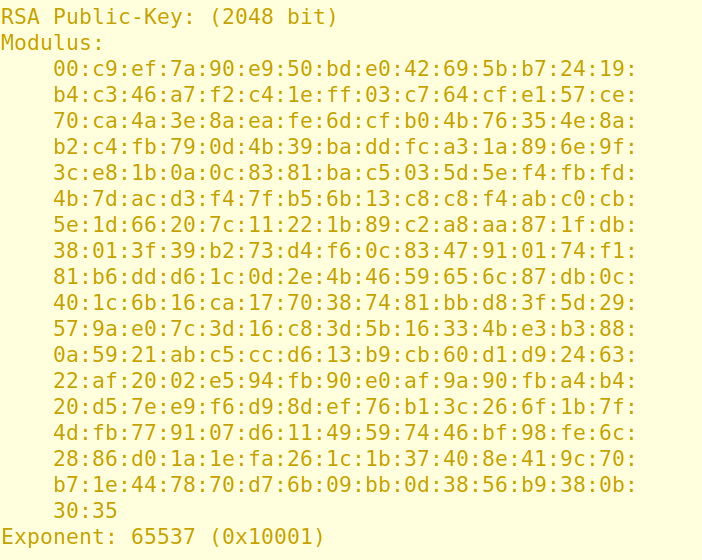
\includegraphics[width=3in]{imgs/rsaPublicInform.png}
\end{center}
\end{frame}

\begin{frame}
\frametitle{Removing the armor}

\vskip 2cm

{\color{blue} 
openssl rsa -in giuperPrivateRSA.pem \\
\qquad\qquad-out giuperPrivateRSANonArmor.pem
}

\end{frame}

\begin{frame}
\frametitle{Encrypting using the RSA public key}

Generate a 16-byte AES key and store it in {\tt aaa.txt}

\vskip .5cm
Encrypt it using RSA

\vskip 1.5cm

{\color{blue}\tt
openssl rsautl -encrypt -oaep -pubin \\

\qquad -inkey giuperPublicRSA.pem -in aaa.txt -out aaa.txt.cpt
}
\end{frame}

\begin{frame}
\frametitle{Decrypting using the RSA private key}

Decrypt the file {\tt aaa.txt.cpt}

\vskip 1.5cm

{\color{blue}\tt
openssl rsautl -decrypt -oaep -inkey giuperPrivateRSA.pem \\

\qquad\qquad -in aaa.txt.cpt -out aaa.txt.new
}
\end{frame}

\begin{frame}
\frametitle{Signing using the RSA private key (Obsolete)}

Signing the file {\tt aaa.txt}

\vskip 1.5cm

{\color{blue}\tt
openssl rsautl -sign -inkey giuperPrivateRSA.pem \\
\qquad\qquad -in aaa.txt -out aaa.txt.sig
}


\vskip 1cm

{\color{brown}
The output file {\tt aaa.txt.sig} contains the file {\tt aaa.txt} and
the signature.
}

\vskip .4cm
Hashing algorithm: MD5
\end{frame}

\begin{frame}
\frametitle{Verifying a signature using the RSA public key (Obsolete)}

Verifying the signature {\tt aaa.txt.sig}

\vskip 1.5cm

{\color{blue}\tt
openssl rsautl -verify -pubin -inkey giuperPublicRSA.pem\\
\qquad\qquad -in aaa.txt.sig -out aaa.txt.vrf
}

\vskip 1cm

{\color{brown}
The output file {\tt aaa.txt.sig} is assumed to contain the file 
{\tt aaa.txt} and the signature.

}
\end{frame}

\begin{frame}
\frametitle{Signing using the RSA private key}

Signing the file {\tt aaa.txt}

\vskip 1.5cm

{\color{blue}\tt
openssl dgst -sha256 -sign giuperPrivateRSA.pem \\
\qquad\qquad -out aaa.txt.sig aaa.txt
}


\vskip 1cm

{\color{brown}
The output file {\tt aaa.txt.sig} does {\bf not} contain
the file {\tt aaa.txt} but only the signature.
}

\vskip .4cm
Hashing algorithm: to be specified (SHA256 in the example)
\end{frame}

\begin{frame}
\frametitle{Verifying a signature using the RSA public key}

Verifying the signature {\tt aaa.txt.sig}

\vskip 1.5cm

{\color{blue}\tt
openssl dgst -sha256 -verify giuperPublicRSA.pem  \\
\qquad\qquad -signature aaa.txt.sig aaa.txt
}

\vskip 1cm

{\color{brown}
The output file {\tt aaa.txt.sig} is not assumed to contain the file 
{\tt aaa.txt} but only the signature. 

\vskip .3cm
The file {\tt aaa.txt} containing the document must be specified in the command.

}
\end{frame}

\begin{frame}
\frametitle{Generating Keys for DSA}

\begin{block}{A two-step process}
\begin{itemize}
\item First we generate the parameters
        
    {\tt\color{magenta} openssl genpkey -genparam -algorithm DSA}
    
    {\color{blue} options:}
    \begin{itemize}
        \item length of $p$ in bits: {\color{magenta}\tt -pkeyopt dsa\_paramgen\_bits: 2048}
        \item length of $1$ in bits: {\color{magenta}\tt -pkeyopt dsa\_paramgen\_q\_bits: 256}
        \item the hashing algorithm: {\color{magenta}\tt -pkeyopt dsa\_paramgen\_md: sha256}
        \item the file containg the parameters: {\color{magenta}\tt -out}
    \end{itemize}

\vskip .2cm

\item Then each user generates his/her pair of keys

       {\color{magenta}\tt openssl genpkey}
        
    {\color{blue} options:}
        \begin{itemize}
            \item the armor algorithm: {\color{magenta}\tt -aes128} 
            \item the file with the parameters {\color{magenta}\tt -paramfile}
            \item the file that will contain the private key {\color{magenta}\tt -out }
    \end{itemize}
\end{itemize}
\end{block}
\end{frame}

\begin{frame}
\begin{center}
\frametitle{What is in a private key?}
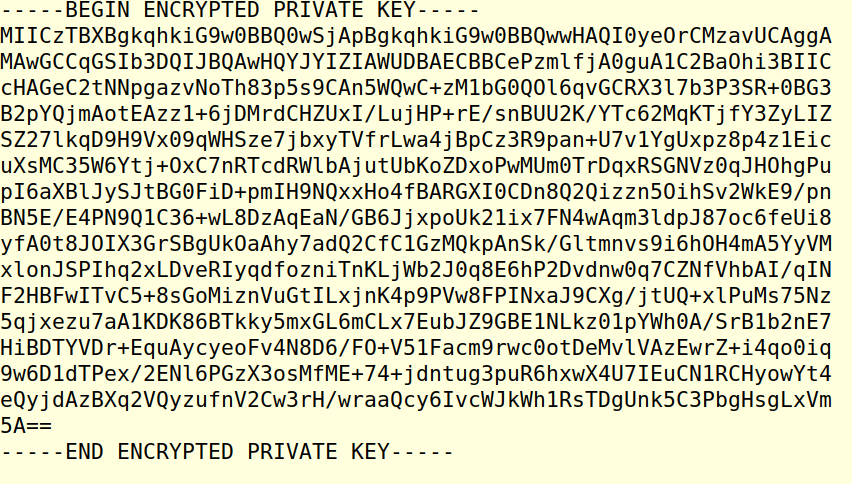
\includegraphics[width=3.5in]{imgs/dsaPrivateRAW.png}
\end{center}
\vfill
Same format as the RSA private key
\end{frame}

\begin{frame}
\frametitle{Inspecting the DSA key}

Same command used for inspecting an RSA key:

\centerline{\color{magenta} openssl pkey -in giuperPrivateDSA.pem -text -noout}

\vfill
\begin{center}
\includegraphics[width=2.5in]{imgs/dsaPrivate.png}
\end{center}
\end{frame}

\begin{frame}
\frametitle{Extracting the public key from the private key}
\vfill
\centerline{\color{magenta} openssl dsa -in giuperPrivateDSA.pem -out giuperPublicDSA.pem -pubout}
\vfill

\end{frame}

\begin{frame}
\frametitle{How to sign and verify using DSA}

\begin{itemize}
\item Sign:

\begin{itemize}
\item {\tt \color{magenta} 
    openssl dgst -sha256 -sign giuperPrivateDSA.pem -out signatureFile documentFile.txt
}
\end{itemize}
\vskip 1cm
\item Verify:
\begin{itemize}
\item {\tt \color{magenta} 
openssl dgst -sha256 -verify giuperPublicDSA.pem -signature signatureFile documentFile.txt
}
\end{itemize}
\end{itemize}
\end{frame}

\begin{frame}
\frametitle{Generating Keys for ECDSA}

\begin{block}{A two-step process}
\begin{itemize}
\item First we generate the parameters
        
    {\tt\color{magenta} openssl genpkey -genparam -algorithm EC}
    
    {\color{blue} options:}
    \begin{itemize}
        \item specify the curve: {\color{magenta}\tt -pkeyopt ec\_paramgen\_curve: secp256k1}
        \item the file containg the parameters: {\color{magenta}\tt -out}
    \end{itemize}

\vskip .2cm

\item Then each user generates his/her pair of keys

       {\color{magenta}\tt openssl genpkey}
        
    {\color{blue} options:}
        \begin{itemize}
            \item the armor algorithm: {\color{magenta}\tt -aes128} 
            \item the file with the parameters {\color{magenta}\tt -paramfile}
            \item the file that will contain the private key {\color{magenta}\tt -out }
    \end{itemize}
\end{itemize}
\end{block}
\end{frame}

\begin{frame}
\frametitle{Inspecting the ECDSA key}

Same command used for inspecting an RSA key:

\centerline{\color{magenta} openssl pkey -in giuperPrivateECDSA.pem -text -noout}

\vfill
\begin{center}
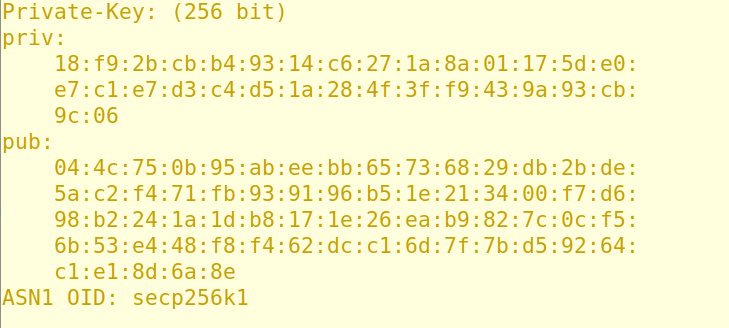
\includegraphics[width=2.5in]{imgs/ecdsaPrivate.png}
\end{center}

399 bytes vs 1194 bytes (DSA) vs 1874 bytes (RSA)

\end{frame}

\begin{frame}
\frametitle{How to sign and verify using ECDSA}

\begin{itemize}
\item Sign:

\begin{itemize}
\item {\tt \color{magenta} 
    openssl dgst -sha256 -sign giuperPrivateECDSA.pem -out signatureFile documentFile.txt
}
\end{itemize}
\vskip 1cm
\item Verify:
\begin{itemize}
\item {\tt \color{magenta} 
openssl dgst -sha256 -verify giuperPublicECDSA.pem -signature signatureFile documentFile.txt
}
\end{itemize}
\end{itemize}
\end{frame}

\end{document}
